\chapter{Modelling, Data, and Simulation}
\label{cha:model}

\minitoc

After describing the state-of-the-art, this Section presents the models, data, and simulation tools used in this thesis. First, we focus on the model describing the offline and online modules. We explain what kind of information is exchanged between offline and online. Also, we detail the power, scheduling, and server decisions. After the model, we introduce the traces used in the experiments. These traces emulates a real environment regarding workload, weather, and platform. Finally, we demonstrate the simulation tools.

\section{Model}

As presented in Chapter \ref{cha:related_work}, a gap in the state-of-the-art is the mix of offline and online. Figure \ref{fig:model} illustrates the architecture proposed by the Datazero2 project, mixing both decision levels \cite{Datazero}. Since this work is part of the Datazero2 project, we use the same architecture. There are four main modules: IT Decision Module (ITDM), Power Decision Module (PDM), Negotiation Module (NM), and Online Decision Module (ODM). ITDM, PDM, and NM are responsible for the offline decisions, and ODM manages the online actions. This thesis focuses on the Online Decision Module, but we present in the following sections the optimizations made in offline modules to provide the data needed by ODM. 

\begin{figure}[!htb]
    \centering
    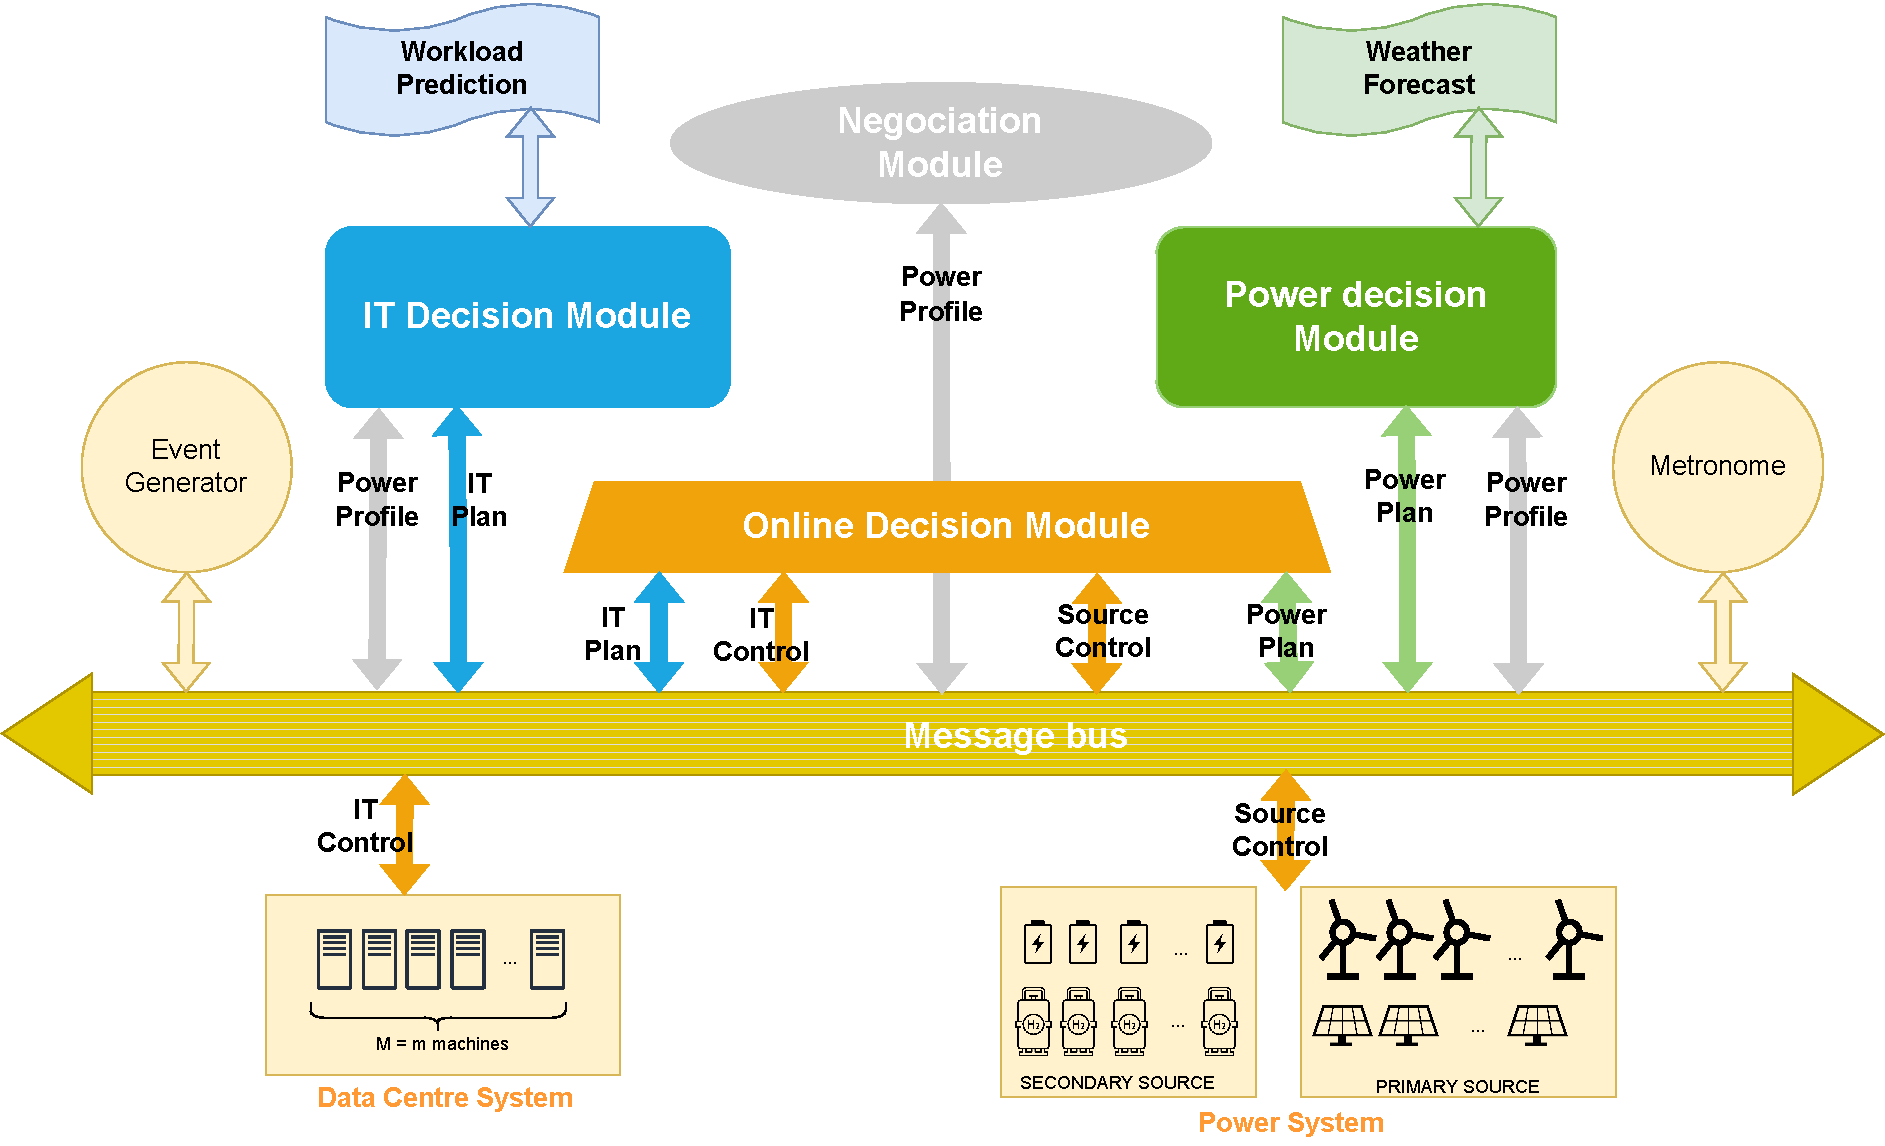
\includegraphics[scale=0.45]{Images/Model/model.pdf}
    \caption{Datazero2 architecture \cite{Datazero}.}
    \label{fig:model}
\end{figure}

Besides these four modules, Datazero2 also includes an event generator and metronome. Both components are essential for the simulations. Event generator simulates the real events of a data center, such as job submission, weather conditions, etc. It simply reads a file and sends the data to the bus. The metronome synchronizes the simulation, managing the clock. So, every component waits for the time evolution from the metronome. This thesis does not detail these components, concentrating on the decision modules and their interactions.

The notations used in the following sections are consolidated in Table \ref{tab:notation}. Both offline and online use the time division from Figure \ref{fig:time_window}. The time window is the horizon of the offline plan. Offline considers the time window to define how far to predict weather and workload. Also, it uses the time window to determine the power and server configuration plan duration. Our model divides the time window into several time steps, as represented in Figure \ref{fig:time_window} by the different $t$. The actions for power and server are constant inside the time step. For example, if a server is at some state in step $t=0$, it will remain at this state during the step duration.

\begin{table}[!htb]
\centering
% \scriptsize
\caption{Notations.}
\label{tab:notation}
\begin{tabular}{l|l}
    \hline
    Notation & Description \\\hline\hline
    % System
    $t$ & Time step (int)\\
    $T$ & Last time step (int)\\
    $\Delta t$ & Time step length (s)\\
    $T_{w}$ & Time window length (s)\\
    % Power
    $P_{prod}$ & Power production by all sources (kW)\\
    $P_{wt}$ & Power delivered by wind turbines (kW)\\
    $P_{pv}$ & Power delivered by solar panels (kW)\\
    $P_{fc}$ & Power delivered by fuel cell (kW)\\
    $P_{ez}$ & Power put into electrolyzer to generate hydrogen (kW)\\
    $P_{dch}$ & Battery discharging power (kW)\\
    $P_{ch}$ & Battery charging power (kW)\\
    $SoC(t)$ & State of Charge at instant $t$ (\%)\\
    $LoH(t)$ & Level of Hydrogen (kg)\\
    $SoC_{max}$ & Maximal battery State of Charge (\%)\\
    $SoC_{min}$ & Minimal battery State of Charge (\%)\\
    $LoH_{max}$ & H2 tank limit (kg)\\
    $P_{dch_{max}}$ & Battery maximum discharging power (kW)\\
    $P_{ch_{max}}$ & Battery maximum charging power (kW)\\
    $P_{fc_{max}}$ & Fuel cell maximum charging power (kW)\\
    $P_{ez_{min}}$ & Electrolyzer minimum charging power (kW)\\
    $P_{ez_{max}}$ & Electrolyzer maximum charging power (kW)\\
    $SoC_{target}$ & Target State of Charge at the end of the time window (\%)\\
    $LoH_{target}$ & Target Level of Hydrogen at the end of the time window (kg)\\
    $rf$ & Relax factor (float) \\
    $P_{load}$ & Estimated power demand (kW)\\
    % IT
    \hline
\end{tabular}
\end{table}

\begin{figure}[!htb]
    \centering
    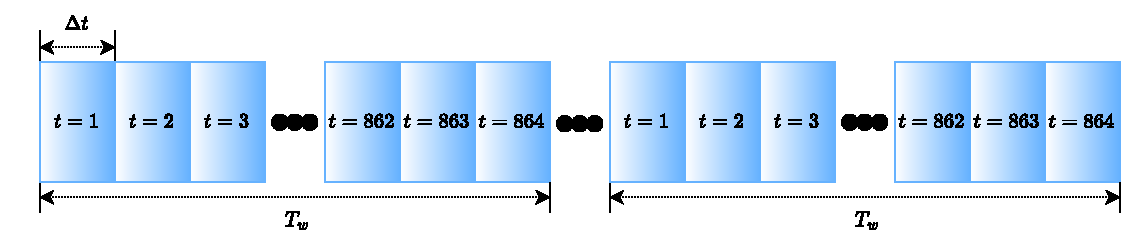
\includegraphics[scale=0.75]{Images/Model/Time window.pdf}
    \caption{Time window definition.}
    \label{fig:time_window}
\end{figure}

\subsection{Offline Decision Modules}
This section starts presenting the offline decision module. First, we demonstrate how PDM and ITDM agree on a power envelope (through NM). Then, we explain the power decisions from PDM, resulting in a power plan. Finally, we detail the ITDM, which defines the IT plan.

\subsubsection{Negotiation (NM)}
Negotiation is a crucial step in Datazero2 architecture. A renewable-only data center introduces several constraints and decision variables. On the PDM side, it must approximate demand and production while considering long-term storage elements. For example, PDM can provide more power from hydrogen in a case with low renewable generation. However, PDM must evaluate the impact of its actions since the energy of the storage is finite. On the other hand, ITDM maximizes the Quality of Service. Thus, it demands more energy to run more servers at faster speeds. NM is between PDM and ITDM, trying to find an agreement. NM works iteratively. On each iteration, both PDM and ITDM propose a power envelope to NM, considering the objective of each module. A power envelope is a time series of the power production from the sources in a time window. While PDM tries to reduce the power envelope to control the storage, ITDM increases it to run more jobs faster. NM compares both envelope propositions and returns a new one. Then, each module verifies if they can use the proposed power envelope. They run several iterations until both agree or reach a timeout.

Since this thesis focus on the online part, we simplify this process. We implemented the negotiation in three steps. First, ITDM proposes a power envelope $P_{load}$ based on the energy demanded to run a predicted workload. Then, PDM takes this envelope and runs its optimization. It can degrade the power envelope to meet its objectives, resulting in a new power envelope $P_{prod}$. Finally, ITDM takes the PDM power production and finds the best server configuration that meets it. The following sections present the PDM and ITDM optimizations.

\subsubsection{Power Decision Module (PDM)}
PDM plans the renewable source engagement to provide the energy needed to maintain the IT elements. A renewable-only data center introduces several constraints in power generation. Therefore, PDM must approximate the demanded power while considering long-term storage elements. For example, it can use more energy coming from hydrogen during the winter, which has lower power production, compensating for this usage in the summer, which has higher power generation. On the other hand, PDM can degrade the provided energy due to a lack of energy from storage and estimated renewable. In the context of Datazero, \citeauthor{haddad2019mixed} created the first model to solve this problem \cite{haddad2019mixed}. This thesis uses a similar model to PDM. Equation \ref{equ:model_energy} gives the power production from all renewable sources. $P_{wt}(t)$, $P_{pv}(t)$, $P_{fc}(t)$, $P_{ez}(t)$, $P_{dch}(t)$, and $P_{ch}(t)$ are calculated using Equations \ref{equ:wind_turbines}, \ref{equ:panel_solar_with_temperature}, \ref{equ:hydrogen_full_cell}, \ref{equ:hydrogen_electrolyzer} and \ref{equ:battery_energy} from Section \ref{sec:related_work_electrical_elements}.  

\begin{equation}
    \label{equ:model_energy}
    P_{prod}(t) = P_{wt}(t) + P_{pv}(t) + (P_{fc}(t) + P_{dch}(t) - P_{ez}(t) - P_{ch}(t)), \quad \forall 0 \le t \le T
\end{equation}

$P_{ch}(t)$, $P_{dch}(t)$, $P_{ez}(t)$, and $P_{fc}(t)$ are the decision variables in Equation \ref{equ:model_energy}, since $P_{wt}(t)$ and $P_{pv}(t)$ come from wind speed and solar irradiation. As presented in Section \ref{sec:related_work_electrical_elements}, $SoC(t)$ depends on the charge $P_{ch}(t)$ and discharge $P_{dch}(t)$ (see Equation \ref{equ:battery_energy}), and $LoH(t)$ depends on the power of the electrolyzer $P_{ez}(t)$ and fuel cells $P_{fc}(t)$ (see Equation \ref{equ:hydrogen_level}). Regarding $SoC(t)$, the state of charge must be between the boundaries $SoC_{min}$ and $SoC_{max}$, as demonstrated in Equation \ref{equ:battery_boundaries}. These boundaries help to extend the battery life \cite{xu2016modeling}.

\begin{equation}
    \label{equ:battery_boundaries}
    SoC_{min} \leq SoC(t) \leq SoC_{max}, \quad \forall 0 \le t \le T
\end{equation}

On the other hand, hydrogen only has the tank size as a boundary. So, Equation \ref{equ:hydrogen_boundaries} presents the level of hydrogen constraint.

\begin{equation}
    \label{equ:hydrogen_boundaries}
    0 \leq LoH(t) \leq LoH_{max}, \quad \forall 0 \le t \le T
\end{equation}

Considering the power to charge/discharge, both have upper limits. These boundaries avoid destroying the battery. So, we introduce constraints \ref{equ:discharge_boundary} and \ref{equ:charge_boundary}.

\begin{equation}
    \label{equ:discharge_boundary}
    0 \leq P_{dch}(t) \leq P_{dch_{max}}, \quad \forall 0 \le t \le T
\end{equation}

\begin{equation}
    \label{equ:charge_boundary}
    0 \leq P_{ch}(t) \leq P_{ch_{max}}, \quad \forall 0 \le t \le T
\end{equation}

Fuel cells and electrolyzers also have boundaries. While fuel cells have only a maximum limit, electrolyzers have an operating range. So, Equations \ref{equ:fuelcells_boundary} and \ref{equ:electrolyzer_boundary} present them.

\begin{equation}
    \label{equ:fuelcells_boundary}
    0 \leq P_{fc}(t) \leq P_{fc_{max}}, \quad \forall 0 \le t \le T
\end{equation}

\begin{equation}
    \label{equ:electrolyzer_boundary}
    P_{ez_{min}} \leq P_{ez}(t) \leq P_{ez_{max}}, \quad \forall 0 \le t \le T
\end{equation}

Another important constraint is the target hydrogen and battery level at the end of the time window. Using only the previous constraints, the model can use all the power available in the energy storages, drying them but providing a high quality of service. However, Figure \ref{fig:time_window} shows that the time windows are chained. So, the next time window will not have energy in the storage. Therefore, we introduce these targets. So, the state of charge and level of hydrogen in the last step of the time window must respect Equations \ref{equ:soc_target} and \ref{equ:loh_target}. These targets can be the subject of another optimization or indicated by hand by the data center manager. Also, the targets must consider the long-term perspective, such as seasons with lower/higher production, the peak of demand over an external event, etc. 

\begin{equation}
    \label{equ:soc_target}
    SoC(T) \ge SoC_{target}
\end{equation}

\begin{equation}
    \label{equ:loh_target}
    LoH(T) \ge LoH_{target}
\end{equation}

Finally, the objective is to approximate the power production to the power demand. So, Equation \ref{equ:load_production} shows the relation between demand ($P_{load}$) and generation ($P_{prod}$). The optimization finds a solution where the production is higher or equal to the demand. However, it can not match both in every case. Therefore, the model introduces a demand degradation using a relax factor ($rf$). With the relax factor equal to 0, it matches demand and production. Increasing the relax factor would reduce the power given to IT, impacting the QoS. Thus, the objective is reducing the relax factor, as presented in Equation \ref{equ:objective_function}.

\begin{equation}
    \label{equ:load_production}
    P_{prod}(t) \ge (1 - rf) \times P_{load}
\end{equation}

\begin{equation}
    \label{equ:objective_function}
    minimize\ rf
\end{equation}

\citeauthor{haddad2019mixed} presented a way to linearize this model, allowing it to be solved using MILP. This thesis used the \citeauthor{haddad2019mixed} proposition to solve it using MILP. 

% \begin{equation}
%     \label{equ:model_wind_turbines}
%     P_{WT}(t) = \begin{cases}
%         0 & v \leq v_{in} \text{ or } v(t) > v_{out} \\
%         P_{WT,rated} \times \frac{v^{3}(t) - v^{3}_{in}}{v^{3}_{rated} - v^{3}_{in}} & v_{in} < v(t) \leq v_{rated} \\
%         P_{WT,rated} & v_{rated} < v(t) \leq v_{out}
%     \end{cases}
% \end{equation}

% \begin{equation}
%     \label{equ:model_panel_solar_with_temperature}
%     P_{pv}(t) = P_{R,PV} \times (R / R_{ref}) \times \eta_{PV}
% \end{equation}

% \begin{equation}
%     \label{equ:model_battery_energy}
%     E_{bat}(t) = (E_{bat}(t-1) \times (1 - \sigma)) + (P_{ch}(t-1) \times \eta_{ch} \times \Delta t) - (P_{dch}(t-1) \times \eta_{dch} \times \Delta t)
% \end{equation}
% \begin{equation}
%     \label{equ:model_battery_state_of_charge}
%     SoC(t) = \frac{E_{bat}(t)}{B_{size}} \times 100
% \end{equation}

% \begin{equation}
%     \label{equ:model_hydrogen_electrolyzer}
%     P_{ez}(t) \times \Delta t = \frac{HH_{h_{2}} \times Q_{ez}(t)}{\eta_{ez}}
% \end{equation}

% \begin{equation}
%     \label{equ:model_hydrogen_full_cell}
%     P_{fc}(t) \times \Delta t = LH_{h_{2}} \times Q_{fc}(t) \times \eta_{fc}
% \end{equation}

% \begin{equation}
%     \label{equ:model_hydrogen_level}
%     LoH(t) = LoH(t-1) + Q_{ez}(t-1) - Q_{fc}(t-1)
% \end{equation}

\subsubsection{IT Decision Module (ITDM)}

Following PDM optimization, ITDM aims to maximize QoS, defining the server configuration. Server configuration means the CPU p-state of the servers and state (sleep). For each p-state, the server has a speed (in flop per second, flops) and power consumption (in W). Table \ref{tab:servers} exemplifies this relation. The CPU frequency range is discrete, although some works define it to be continuous~\cite{saha2012experimental}. 

\begin{table}[!htb]
\centering
\caption[Server definition example]{Server definition example. The power is for all server's processors busy. The values are from Grid5000's Parasilo server~\cite{dacosta:hal-03453537v1, dacostakeynote}.}
\label{tab:servers}
\begin{tabular}{c|c|c}
    \hline
    State        & Power (W) & Speed (Gflops) \\ \hline\hline
    0                       & 221.77                   & 38.4                          \\
    1                       & 216.77                   & 37.78                         \\
    2                       & 213.58                   & 36.93                         \\
    3                       & 208.90                   & 36.01                         \\
    4                       & 204.45                   & 34.72                         \\
    5                       & 200.62                   & 33.90                         \\
    6                       & 197.28                   & 32.84                         \\
    7                       & 192.49                   & 31.72                         \\
    8                       & 184.26                   & 30.63                         \\
    9                       & 182.04                   & 29.25                         \\
    10                      & 179.75                   & 27.93                         \\
    11                      & 176.70                   & 26.37                         \\
    12                      & 175.53                   & 25.01                         \\
    13 (sleep)              & 4.5                      & 0                             \\ \hline
\end{tabular}
\end{table}

\subsection{Offline Plan}

\subsection{Online Decision Modules}

\subsubsection{Job scheduling}

\subsubsection{Modifying Power Plan}

\subsubsection{Modifying IT Plan}

\section{Data}

\subsection{Workload Trace}

% Talk about noise

\subsection{Weather Trace}

% Talk about noise

\subsection{Platform Configuration}

\section{Simulation}

\subsection{Simulator}

\subsection{Metrics}

\subsection{Datazero2 Middleware}
% Explain about docker

\section{Conclusion}